\clearpage
\section{Discussion}

The results obtained from empirical measurements in section \ref{section:performance_analysis} are consistent and show that the first prototype of the system doesn't perform optimally and therefore can't be approved. On the other hand, the tests performed using a zero input signal were promising and showed that the system has the potential to be very good. Also the fix implemented by the hardware team shows promising results and it's very probable that the second prototype will fulfill the requirements set for it. The fact that the transmitter exhibits a constant SNR of 115 dB, high compared to the 100 dB of the receiver, leads to the assumption that once the receiver is fixed the total system performance will resemble the first prototype's performance measured with zero current. The following speculations are based on this prerequisite.

\subsection{Power vs.\ Performance Trade-Off}

When using a fixed \spo standard deviation limit the minimum measurable IR modulation is the best indicator of system performance -- it sets the actual operating limit of the device. Figure \ref{fig:noise_vs_mod} shows the maximum noise level of the system to reliably measure \spo from a signal with a certain IR modulation, and if it's assumed that the system performance after the ADC buffer fix will be as good as the measurements done with a zero signal, those measurement results can be used to estimate the total system power needed to achieve a certain noise performance. These two data sets combined provide table \ref{tbl:power_vs_mod} that links system power for a typical patient and minimum measurable IR modulation. It can be seen that system performance is excellent even when using minimal power, although to achieve the best possible performance a lot of power has to be used. This was to be expected as discussed in section \ref{section:pulse_oximetry}. The relationship between power and performance is somewhat a 1/m\subscript{IR} type curve, shown in figure \ref{fig:power_vs_mod}.

\begin{table}[htcb]
  \caption{The relationship between system settings, power and low perfusion performance.}
  \begin{tabular}{|c|c|c|c|c|c|}
  \hline
  \textbf{F\subscript{s} (Hz)} & \textbf{R\subscript{f} (k$\Omega$)} & \textbf{I\subscript{LED} (mA)} & \textbf{P (mW)} & \textbf{$\sigma$ (LSB)} & \textbf{Min m\subscript{IR} (\%)} \\
  \hline
  625 & 50   & 150 & 125 & 9.5 & 0.021 \\
  625 & 100  & 75  & 65  & 9.9 & 0.022 \\
  625 & 250  & 35  & 34  & 13  & 0.029 \\
  225 & 250  & 35  & 16  & 16  & 0.035 \\
  225 & 500  & 20  & 12  & 21  & 0.046 \\
  225 & 1000 & 10  & 9   & 33  & 0.073 \\
  \hline
  \end{tabular}
  \label{tbl:power_vs_mod}
\end{table}

\begin{figure}[htcb]
  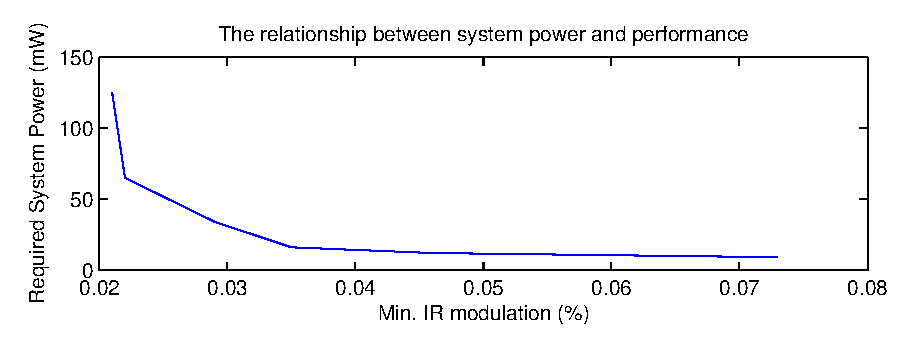
\includegraphics{kuvat/measurements/power_vs_mod.eps}
  \caption{Required system power as a function of IR modulation as listed in table \ref{tbl:power_vs_mod}.}
  \label{fig:power_vs_mod}
\end{figure}

\subsection{Additional Control Parameters}

In previous sections it was assumed that there are no obstructions for controlling the system so that the signal mean always stays around the middle of the ADC range. There can be situations, though, where large gains can't be used due to intense ambient light: as large gain also amplifies the ambient level it could be that the system's dynamic range is too narrow with high gain in some OR applications. Combined with pigmented skin and a thick measurement site it could be that even the selected power mode's maximum current isn't enough to drive the signal to the optimal range. This leads to the fact that measurement SNR drops due to the reduced signal level and has to be taken into account when controlling the system. In effect this is done by measuring the ambient light, setting a maximum gain value based on its level and notifying the host if system performance is limited by the power settings. The host can then decide if it's needed to use more power or not.

\subsection{Using the System as a Stand-Alone Product}

The MSP430 microcontroller has some computing power reserves that aren't used for measurement control. Therefore it could be possible to construct an extremely small and power-efficient solution that does all signal processing using the MSP430. The downside is that since the microcontroller doesn't support hardware division or floating point calculation the algorithm would have to be a heavily stripped-down version with reduced performance. Again, the trade-off between power, size and performance is clear and it's up to the application specifications if the performance provided is enough or not. For example, some home monitoring solutions could do with a very simple algorithm as the patient is not expected to be in a low perfusion state -- such solution would have a greatly extended battery life and improved portability compared to more traditional monitors.
